\chapter{白矮星、中子星与强场物理}
\label{chap:e18}

\begin{chapteropening}
到目前为止，我们打交道的"量子光源"大多是普通恒星：一团热气体，表面温度几千到几万开，发出宽带的热光（第 \ref{chap:e17} 章）。这一章要走到恒星演化的终点站——白矮星（white dwarf）和中子星（neutron star）。它们是把量子物理直接摆到天空上的两个极端标本：白矮星靠电子的\emph{泡利不相容原理}撑着不塌，中子星表面的磁场可以强到让\emph{真空本身}都变成一种有偏振方向的介质。可对我们这些"只会数光子、量相位、测偏振"的观测者来说，它们还带来一个很现实的麻烦：个头太小了。一颗白矮星只有地球那么大，一颗中子星才十几公里——放到几十上百秒差距外，角直径只有微角秒量级，任何单口径望远镜都别想把它"看成一个面"。于是这一章有两条主线拧在一起：一条是\textbf{物理}——简并压、磁层、回旋辐射、真空双折射、表面大气；另一条是\textbf{方法}——既然分辨不了空间结构，我们就改用时间（相位折叠）、能量（能谱）和偏振（Stokes 参量）这三把尺子，把致密天体的信息压进同一张事件表里。这两条线最后都通向后面第 \ref{chap:e22} 章要专门打开的"偏振量子通道"。
\end{chapteropening}


\section{白矮星：电子简并压怎样撑起一颗星}
\label{sec:e18-degeneracy}

先问一个最朴素的问题：一颗恒星烧完了核燃料，没有热核反应再往外顶了，为什么它不干脆一路塌缩成一个点？普通恒星靠的是"热压强"——气体越热，粒子撞得越凶，往外的压力越大。可白矮星已经冷下来了，热运动退居次席。真正顶住引力的，是一种\emph{哪怕温度降到零也不会消失}的压强：电子简并压（electron degeneracy pressure）。它的来历纯粹是量子力学。

物理图像是这样的。把白矮星里的电子想成一群被关在盒子里的乘客，泡利不相容原理（Pauli exclusion principle）规定"一个座位（量子态）最多坐一个（自旋算两个）"。你越是把盒子压小，低能量的座位就越不够坐，后来的电子被迫坐到\emph{动量很高}的座位上去。动量高就意味着运动快、撞墙勤，于是即使一点不加热，这群电子也会拼命往外顶。密度越大，被顶到的动量越高，压强也越大——这就是简并压。

把它写成公式。先算"座位有多满"。在动量空间里，动量小于 \(p\) 的球体体积是 \(\tfrac{4}{3}\pi p^3\)；量子力学告诉我们每个体积为 \(h^3\) 的相空间小格子只能装两个电子（自旋向上、向下各一）。于是单位体积里、动量填到 \(p_F\)（费米动量，Fermi momentum）的电子数密度是
\[
  n_e=\frac{2}{h^3}\cdot\frac{4}{3}\pi p_F^3
     =\frac{8\pi p_F^3}{3h^3}
     =\frac{p_F^3}{3\pi^2\hbar^3},
\]
最后一步用了 \(h=2\pi\hbar\)。反解出费米动量：

\begin{equation}
  p_F=\hbar\,(3\pi^2 n_e)^{1/3},
  \qquad
  n_e=\frac{\rho}{\mu_e m_p}.
  \label{eq:e18-fermi}
\end{equation}
\begin{formulaexplain}
\(p_F\)：费米动量（\(\mathrm{g\,cm\,s^{-1}}\)），电子被填到的最高动量。\(n_e\)：电子数密度（\(\mathrm{cm^{-3}}\)）。\(\rho\)：质量密度；\(\mu_e\)：每个电子摊到的重子数（碳氧星取 \(\simeq2\)）；\(m_p\)：质子质量。密度越高，电子被泡利原理顶得越高。
\end{formulaexplain}

逐符号落地。\(n_e\) 的单位是 \(\mathrm{cm^{-3}}\)；\(\rho\) 是质量密度（\(\mathrm{g\,cm^{-3}}\)）；\(m_p=1.67\times10^{-24}\,\mathrm{g}\)；\(\mu_e\) 之所以出现，是因为白矮星里既有电子也有原子核，每个电子平均"配"了 \(\mu_e\) 个核子的质量，碳氧成分近似 \(\mu_e\simeq2\)。代个真实数字：一颗 \(M\simeq0.6\,M_\odot\)、半径约地球大小（\(R\simeq0.012\,R_\odot\simeq1.3\,R_\oplus\)）的典型 DA 白矮星，平均密度已达 \(10^6\,\mathrm{g\,cm^{-3}}\) 量级，中心可到 \(10^6\)–\(10^9\,\mathrm{g\,cm^{-3}}\)。这个密度是水的百万倍——一茶匙这样的物质有一吨重。

有了 \(p_F\) 就能算压强。理想费米气体的压强来自动量流：\(P=\tfrac13\int_0^{p_F} v(p)\,p\,\dfrac{8\pi p^2}{h^3}\,dp\)，其中 \(\tfrac13\) 是三个方向平摊的几何因子，\(v(p)\) 是动量为 \(p\) 的电子速度。当电子跑得比光慢很多（\(p_F\ll m_ec\)），\(v=p/m_e\)，积分是
\[
  P_{\rm NR}=\frac{8\pi}{3h^3m_e}\int_0^{p_F}p^4\,dp
           =\frac{8\pi\,p_F^5}{15h^3m_e}
           =\frac{p_F^5}{15\pi^2\hbar^3 m_e}.
\]
把 \(\eqref{eq:e18-fermi}\) 的 \(p_F\) 代进去、整理指数，得到

\begin{equation}
  P_{\rm NR}=\frac{(3\pi^2)^{2/3}}{5}\,
             \frac{\hbar^2}{m_e}\,n_e^{5/3}.
  \label{eq:e18-pnr}
\end{equation}
\begin{formulaexplain}
\(P_{\rm NR}\)：非相对论电子简并压（\(\mathrm{dyn\,cm^{-2}}\)），随密度以 \(n_e^{5/3}\) 上冲。这是一支"很硬"的支撑：密度稍升，压强猛增，普通白矮星就靠它顶住引力。
\end{formulaexplain}

请留意那个指数 \(5/3\)。它意味着这支压强"很硬"——你想再压小一点，它就用力得多的反抗。这就是为什么低质量白矮星能安安稳稳地存在几十亿年。

可是质量一大，麻烦就来了。质量越大、压得越紧、\(n_e\) 越高，费米动量就可能超过 \(m_ec\)：电子被顶到\emph{接近光速}。这时 \(v\to c\) 不再是 \(p/m_e\)，速度被光速卡住涨不上去了。把 \(v=c\) 代进同一个压强积分：
\[
  P_{\rm ER}=\frac{8\pi c}{3h^3}\int_0^{p_F}p^3\,dp
           =\frac{2\pi c\,p_F^4}{3h^3}
           =\frac{c\,p_F^4}{12\pi^2\hbar^3},
\]
再代 \(p_F\)：

\begin{equation}
  P_{\rm ER}=\frac{(3\pi^2)^{1/3}}{4}\,\hbar c\,n_e^{4/3}.
  \label{eq:e18-per}
\end{equation}
\begin{formulaexplain}
\(P_{\rm ER}\)：极端相对论电子简并压，密度指数软化为 \(4/3\)。支撑变软后，质量再加，半径急剧缩小——这是走向 Chandrasekhar 极限的物理根源。
\end{formulaexplain}

现在指数从 \(5/3\) 降到了 \(4/3\)。这一降是致命的：压强对密度的响应变"软"了，你再往上加质量，它顶不住多少。极端情形下引力和简并压的密度指数打平，星体失去稳定支撑——这就是 Chandrasekhar 极限（Chandrasekhar mass）的物理来源 \citep{1931ApJ....74...81C,1935MNRAS..95..207C,1961ApJ...134..683H}。

把上面的标度关系接到观测者能用的形式，常写成 Nauenberg 的质量–半径近似：

\begin{equation}
  R\simeq 0.0112\,R_\odot
  \left[\left(\frac{M_{\rm Ch}}{M}\right)^{2/3}
  -\left(\frac{M}{M_{\rm Ch}}\right)^{2/3}\right]^{1/2},
  \qquad
  M_{\rm Ch}\simeq 5.83\,\mu_e^{-2}\,M_\odot .
  \label{eq:e18-nauenberg}
\end{equation}
\begin{formulaexplain}
\(R\)：白矮星半径；\(M\)：质量；\(M_{\rm Ch}\)：Chandrasekhar 极限质量（\(\mu_e=2\) 时约 \(1.46\,M_\odot\)）。\(M\to M_{\rm Ch}\) 时方括号趋零，半径塌向零——"越重越小"。
\end{formulaexplain}

这个式子把\eqref{eq:e18-pnr}、\eqref{eq:e18-per}两支压强合成一条曲线。它假设零温、不转、无强磁场形变，适合估算 \(0.2\)–\(1.35\,M_\odot\) 白矮星的主标度。请注意它和普通恒星\emph{相反}的脾气：普通恒星越重越大，白矮星却越重越小。真实半径还受核心成分、氢氦包层厚度、有限温度和磁场影响，高精度工作要靠演化模型或双星约束 \citep{1972ApJ...175..417N,2017MNRAS.470.4473P,2020ApJ...899..146C}。图~\ref{fig:e18-wd-mr} 把这条"越重越小"的曲线画了出来。

\begin{figure}[tbp]
\centering
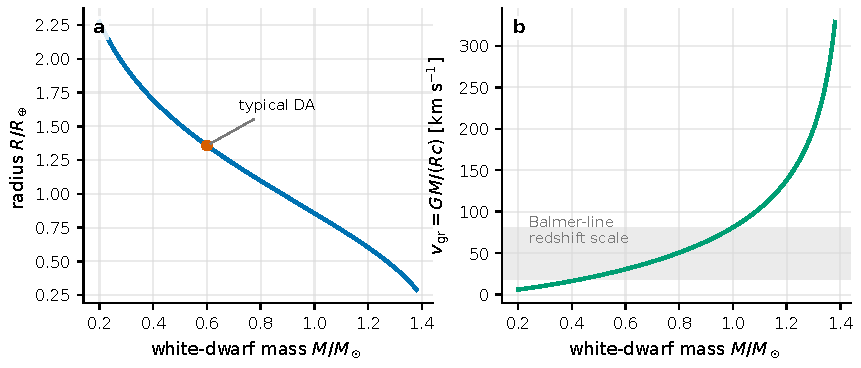
\includegraphics[width=0.94\linewidth]{figures/generated/chapter_11/ch11_white_dwarf_mass_radius.pdf}
\caption{白矮星质量增加时半径变小，靠近 Chandrasekhar 极限时收缩更快。右图把同一质量–半径关系换成光谱中可测的引力红移速度 \(v_{\rm gr}=GM/(Rc)\)，典型 DA 白矮星的 Balmer 线红移是几十 \(\mathrm{km\,s^{-1}}\)，已经接近或超过普通恒星大气运动的速度尺度。}
\label{fig:e18-wd-mr}
\end{figure}


\section{小角尺度：致密天体为什么这么难"看清"}
\label{sec:e18-angsize}

上一节算出白矮星大概只有地球那么大。这一节把这个"小"翻译成观测者最怕的一个量：角直径（angular diameter）。回忆第 \ref{chap:e11} 章讲成像时的定义——一个真实直径为 \(2R\)、距离 \(d\) 的圆盘，张开的角是

\begin{equation}
  \theta_{\rm WD}=\frac{2R}{d}
  \simeq 11\,\mu\mathrm{as}
  \left(\frac{R}{0.012\,R_\odot}\right)
  \left(\frac{10\,\mathrm{pc}}{d}\right).
  \label{eq:e18-theta}
\end{equation}
\begin{formulaexplain}
\(\theta_{\rm WD}\)：白矮星角直径（微角秒 \(\mu\mathrm{as}\)）；\(R\)：半径；\(d\)：距离。即使近到 \(10\,\mathrm{pc}\)，也只有约 \(11\,\mu\mathrm{as}\)——远在单口径望远镜的分辨能力之外。
\end{formulaexplain}

把数字摆出来体会一下。\(1\,\mathrm{rad}=2.06\times10^{11}\,\mu\mathrm{as}\)；\(10\,\mathrm{pc}=3.1\times10^{19}\,\mathrm{cm}\)，\(R=0.012\,R_\odot=8.3\times10^8\,\mathrm{cm}\)。于是 \(\theta=2R/d\approx5.3\times10^{-11}\,\mathrm{rad}\approx11\,\mu\mathrm{as}\)。对照第 \ref{chap:e12} 章：一台 8 米镜在可见光的 Rayleigh 角约 \(16\,\mathrm{mas}=1.6\times10^4\,\mu\mathrm{as}\)（换算用 \(1\,\mathrm{mas}=10^3\,\mu\mathrm{as}\)）——比这颗白矮星大了约三个数量级（\(1.6\times10^4/11\approx1.5\times10^3\)）。就算换 30 米巨镜，Rayleigh 角只缩到约 \(4.3\,\mathrm{mas}\approx4.3\times10^3\,\mu\mathrm{as}\)，仍差两到三个数量级。结论很硬：\textbf{致密天体的空间结构，单口径成像基本无望}。

那怎么办？有两条出路，恰好都是本书前半部搭好的舞台。第一条是把基线拉长——第 \ref{chap:e10} 章的强度干涉（intensity interferometry）测的是两台相距 \(B\) 的望远镜之间的二阶相干 \(g^{(2)}\)，等效分辨本领是 \(\lambda/B\)。要把 \(11\,\mu\mathrm{as}\) 分辨出来，需要 \(B\sim\lambda/\theta\sim5\times10^{-5}\,\mathrm{cm}/5\times10^{-11}\approx10^6\,\mathrm{cm}=10\,\mathrm{km}\) 量级的基线——这正是第 \ref{chap:e22}、\ref{chap:e24} 章工程方案要够的尺度。第二条出路更省事：既然分辨不了"面"，那就别硬碰空间，改去挖\emph{时间}和\emph{偏振}里的信息。致密天体转得快、磁场强，把结构信息大量编码在光变相位和偏振里——这正是本章后面几节的主战场。

顺带说一个"不用分辨就能量物理"的漂亮例子：引力红移。光子从强引力势阱里爬出来会损失能量、波长变长，等效成一个视向速度

\begin{equation}
  v_{\rm gr}=\frac{GM}{Rc}
  \simeq 31.8\,\mathrm{km\,s^{-1}}
  \left(\frac{M}{0.6\,M_\odot}\right)
  \left(\frac{0.012\,R_\odot}{R}\right).
  \label{eq:e18-vgr}
\end{equation}
\begin{formulaexplain}
\(v_{\rm gr}\)：引力红移等效速度，正比于 \(M/R\)（即紧致度）。谱线红移因此把质量–半径关系变成一个可测的速度——不需要分辨星面。
\end{formulaexplain}

推导只有一步：广义相对论给出的分数红移是 \(\Delta\lambda/\lambda\simeq GM/(Rc^2)\)（弱场极限），乘以 \(c\) 就是等效速度 \(v_{\rm gr}=GM/(Rc)\)。它把"越重越小"（\eqref{eq:e18-nauenberg}）的白矮星翻译成谱线上几十 \(\mathrm{km\,s^{-1}}\) 的位移，已经超过普通恒星大气的运动速度，因此可测。当然实测要扣掉系统本动速度、对流线移和 Stark 位移，所以大样本工作常把 Gaia 半径、SDSS 光谱线心和运动学模型一起平均。图~\ref{fig:e18-wd-mr} 右图正是这条"半径换速度"的映射。


\section{磁白矮星：吸积几何怎样写进相位和偏振}
\label{sec:e18-mcv}

有一类白矮星带着强磁场：孤立磁白矮星表面场从 \(10^6\) 到 \(10^9\,\mathrm{G}\)，吸积双星（激变变星，cataclysmic variable）里的极（polar）和中介极（intermediate polar）常见 \(1\)–\(200\,\mathrm{MG}\)。这里磁场不再是配角，它直接把结构问题和光子统计问题拧在一起。先给磁场一个"作用半径"。一个磁偶极子的磁矩是场强乘以半径立方：

\begin{equation}
  \mu = B_* R_{\rm WD}^3
  \simeq 5.1\times10^{33}\,\mathrm{G\,cm^3}
  \left(\frac{B_*}{10\,\mathrm{MG}}\right)
  \left(\frac{R_{\rm WD}}{8\times10^8\,\mathrm{cm}}\right)^3 .
  \label{eq:e18-mu}
\end{equation}
\begin{formulaexplain}
\(\mu\)：磁矩（\(\mathrm{G\,cm^3}\)）；\(B_*\)：表面磁场；\(R_{\rm WD}\)：半径。磁矩越大，磁场就能在离星更远的地方接管吸积流。
\end{formulaexplain}

为什么要算磁矩？因为落向白矮星的气体是电离的，带电粒子只能沿磁力线走。当磁场的能量密度足以主导流的动能时，气流就被"接管"、被迫顺着磁力线拐向磁极。这个接管发生的半径叫磁层半径（magnetospheric radius）：

\begin{equation}
  r_m \simeq k
  \left(\frac{\mu^4}{2GM\dot M^2}\right)^{1/7},
  \label{eq:e18-rm}
\end{equation}
\begin{formulaexplain}
\(r_m\)：磁层半径；\(k\sim0.5\)–\(1\) 是几何因子；\(\dot M\)：吸积率。磁矩越大把磁层推得越远，吸积率越高把磁层压得越近。
\end{formulaexplain}

那个 \(1/7\) 次幂看着古怪，其实来自"磁压等于落流冲压"的平衡：磁压 \(\propto B^2\propto\mu^2/r^6\)，落流冲压 \(\propto\dot M\sqrt{GM/r}/r^2\propto r^{-5/2}\)，两边令相等解出 \(r_m\propto(\mu^4/GM\dot M^2)^{1/7}\)——指数 \(4\)、\(1\)、\(2\) 和 \(7\) 全是这么配平出来的。激变变星的 \(\dot M\) 从 \(10^{-11}\) 到 \(10^{-8}\,M_\odot\,\mathrm{yr^{-1}}\) 不等，磁层大小随之在星面附近到几十倍星半径之间浮动。

磁层大小要和另一个半径比才有意义——共转半径（corotation radius），也就是磁场随星刚性共转的角速度恰好等于开普勒轨道角速度的地方：

\begin{equation}
  r_{\rm co}=\left(\frac{GM}{\Omega_s^2}\right)^{1/3},
  \label{eq:e18-rco}
\end{equation}
\begin{formulaexplain}
\(r_{\rm co}\)：共转半径；\(\Omega_s\)：白矮星自转角速度。此处"磁场拉着转"的速度与"引力允许的绕转"速度打平，是吸积能否顺利落下的分水岭。
\end{formulaexplain}

它的推导也是一步：令共转线速度对应的离心力 \(\Omega_s^2 r\) 等于引力 \(GM/r^2\)，解出 \(r_{\rm co}=(GM/\Omega_s^2)^{1/3}\)。物理判据很直观：若 \(r_m<r_{\rm co}\)，物质在共转半径以内被磁场接手，可以较顺当地沿磁力线落到磁极；若 \(r_m\gtrsim r_{\rm co}\)，磁力线在接手处已经转得比开普勒还快，会\emph{甩}物质，形成"螺旋桨"式的抛射或改变流形态。观测上，中介极的 \(P_{\rm spin}/P_{\rm orb}\) 常在 \(0.01\)–\(0.6\)，而极几乎同步（\(P_{\rm spin}\simeq P_{\rm orb}\)）\citep{1970ApJ...160L.147A,2000PASP..112..873W,1991MNRAS.249..460W,2008ApJ...672..524N}。图~\ref{fig:e18-mcv-map} 把这套"磁矩与自转快慢决定几何"的分类画了出来。

\begin{figure}[tbp]
\centering
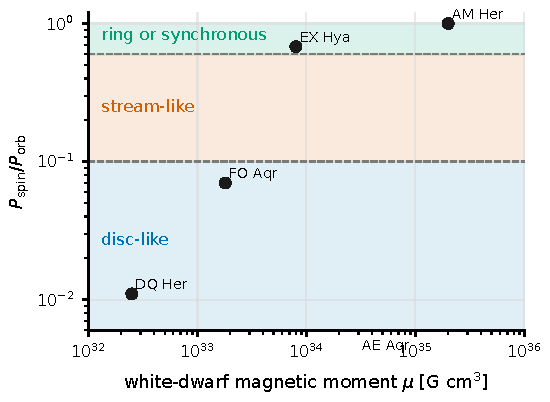
\includegraphics[width=0.78\linewidth]{figures/generated/chapter_11/ch11_magnetic_cv_flow_map.pdf}
\caption{磁激变变星的吸积流主要由白矮星磁矩和自转相对轨道的快慢决定。低 \(P_{\rm spin}/P_{\rm orb}\) 系统容易形成盘状流，中间区域常出现磁控流，接近同步或高比值系统会转向环状、流状或极系统几何；这些几何会直接改变光变相位、圆偏振和相关函数。}
\label{fig:e18-mcv-map}
\end{figure}

流落下来会释放引力势能，转成光。数量级由势阱深度乘以质量流率给出：

\begin{equation}
  L_{\rm acc}\simeq \frac{GM\dot M}{R_{\rm WD}}
  \simeq 1.0\times10^{33}\,\mathrm{erg\,s^{-1}}
  \left(\frac{M}{0.8\,M_\odot}\right)
  \left(\frac{\dot M}{10^{-10}M_\odot\,\mathrm{yr^{-1}}}\right)
  \left(\frac{8\times10^8\,\mathrm{cm}}{R_{\rm WD}}\right).
  \label{eq:e18-lacc}
\end{equation}
\begin{formulaexplain}
\(L_{\rm acc}\)：吸积光度（\(\mathrm{erg\,s^{-1}}\)），等于单位时间释放的引力势能 \(GM\dot M/R\)。它给出这类系统可用光子率的数量级；光学只接收其中一部分。
\end{formulaexplain}

这份光度是各种成分的混合：吸积盘、磁极附近的热斑、柱状冲击区、被照亮的白矮星面，以及\emph{回旋辐射}（cyclotron emission）。这里就接上了本章的一个教学重点——强磁场怎样把偏振写进光里。带电电子在磁场里会绕着磁力线打转，转动的角频率是回旋频率（cyclotron frequency）
\[
  \omega_c=\frac{eB}{m_e c},
  \qquad
  \hbar\omega_c\approx 11.6\,\mathrm{keV}\left(\frac{B}{10^{12}\,\mathrm{G}}\right).
\]
电子转圈就是一个加速的电荷，会辐射；辐射集中在 \(\omega_c\) 及其谐波上。对磁白矮星 \(B\sim10\)–\(200\,\mathrm{MG}=10^7\)–\(2\times10^8\,\mathrm{G}\)，基频光子能量 \(\hbar\omega_c\sim0.1\)–\(2\,\mathrm{eV}\)，加上若干谐波，正好落在近红外到光学——这就是为什么极的光学光变里会鼓起一串"回旋驼峰"。关键在于：电子绕磁力线转，辐射天然带\emph{偏振}——你顺着磁力线看到的是圆偏振，侧着看到的是线偏振。于是偏振成了把回旋成分从盘光、黑体光里\emph{挑出来}的探针。（把非相对论的回旋辐射换成相对论电子，就是第 \ref{chap:e16} 章讲过的同步辐射 synchrotron，两者是同一机制在不同能段的两副面孔。）

偏振怎么读几何？两条经验规则很好用。其一，圆偏振的\emph{符号}如果随自转相位翻转，通常意味着视线扫过了不同的磁极、或磁场投影方向变了号。其二，线偏振峰和总光变峰如果\emph{不同步}，说明"最亮的区域"和"磁场几何最特殊的区域"不是同一块——强度峰来自冲击区加热，偏振峰来自磁场投影。

这些相位调制该怎样在事件表里定量？把光子按白矮星自转相位 \(\phi_s\) 分箱，在每个相位窗内算二阶强度相关（第 \ref{chap:e08} 章的 \(g^{(2)}\)）：

\begin{equation}
  g^{(2)}_{\phi_s}(\tau)=
  \frac{\langle I_{\phi_s}(t)\,I_{\phi_s}(t+\tau)\rangle}
       {\langle I_{\phi_s}(t)\rangle^2}.
  \label{eq:e18-g2phi}
\end{equation}
\begin{formulaexplain}
\(g^{(2)}_{\phi_s}(\tau)\)：固定自转相位窗 \(\phi_s\) 内的二阶强度相关；\(I_{\phi_s}\)：该窗内的计数率。它抽取同一磁极或同一段吸积流在延迟 \(\tau\) 上的"短时记忆"。
\end{formulaexplain}

读法要小心时间尺度。若 \(\tau\) 在毫秒到秒，\(g^{(2)}\) 的结构可能来自冲击区冷却、磁控团块，或者纯属探测器死时间的假信号；若 \(\tau\) 在几十秒到分钟，则更像经典的闪烁（flickering）或大气透明度起伏，而非致密源本身。还有一条铁律：\eqref{eq:e18-g2phi} 里的平均\emph{必须}在同一相位窗、同一能段、同一偏振通道内做，否则轨道调制会被误当成短时相关——这正是"相位分辨"四个字的分量所在。


\section{中子星：磁层怎样切成一张相位事件表}
\label{sec:e18-nsphase}

中子星比白矮星还小一个数量级：半径只有 \(10\)–\(14\,\mathrm{km}\)，质量却常在 \(1.2\)–\(2.2\,M_\odot\)。这么小的天体转得飞快、磁场极强，于是它的磁层被自转"切"成了一套天然的相位坐标。最基本的一条界线是光柱半径（light cylinder radius）——刚性共转的线速度恰好达到光速的地方：

\begin{equation}
  R_{\rm LC}=\frac{c}{\Omega}=\frac{cP}{2\pi}
  \simeq 1.6\times10^3\,\mathrm{km}
  \left(\frac{P}{33\,\mathrm{ms}}\right).
  \label{eq:e18-rlc}
\end{equation}
\begin{formulaexplain}
\(R_{\rm LC}\)：光柱半径；\(P\)：自转周期；\(\Omega=2\pi/P\)：角速度。此处 "跟着星刚性共转" 需要达到光速，因此它是开放磁力线、粒子加速与高能辐射能组织的最外边界。
\end{formulaexplain}

推导只有一句话：共转线速度 \(v=\Omega r\) 令其等于 \(c\)，解出 \(r=c/\Omega=cP/2\pi\)。数量级很有画面感：Crab 脉冲星 \(P\simeq33\,\mathrm{ms}\)，光柱约 \(1600\,\mathrm{km}\)；毫秒脉冲星 \(P\simeq1.5\)–\(10\,\mathrm{ms}\)，光柱只有几十到几百公里；磁星（magnetar）\(P\simeq2\)–\(12\,\mathrm{s}\)，光柱可达 \(10^5\,\mathrm{km}\) 以上。在 \(R_{\rm LC}\) 以内的磁力线闭合、随星共转；越过它就得开放，粒子沿开放磁力线加速、辐射。脉冲星的发现和"旋转中子星"解释确立了这幅图像，Crab 又把旋转能损失和超新星遗迹联系起来 \citep{1968Natur.217..709H,1968Natur.218..731G,1968Natur.219..145P,1972ApJ...175..217B}。图~\ref{fig:e18-lc} 画出光柱随周期的线性增长和 Crab 型相位轮廓。

\begin{figure}[tbp]
\centering
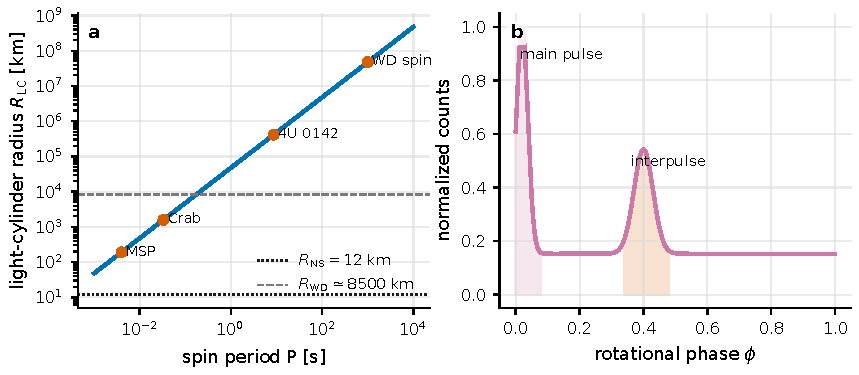
\includegraphics[width=0.94\linewidth]{figures/generated/chapter_11/ch11_light_cylinder_phase.pdf}
\caption{光柱半径随自转周期线性增加。毫秒脉冲星的光柱只有几十到几百公里，Crab 约 \(1.6\times10^3\,\mathrm{km}\)，磁星则可到 \(10^5\,\mathrm{km}\) 以上。右图是 Crab 型相位折叠轮廓，主脉冲和 interpulse 的相位窗决定哪些光子进入后续的强度相关或偏振统计。}
\label{fig:e18-lc}
\end{figure}

磁场强到什么程度？我们量不到中子星表面，但可以从它转得越来越慢反推。一个磁化的转动天体像个天线，向外辐射磁偶极波、带走能量，于是自转减慢。这一步的中间桥梁是磁偶极辐射公式：一个磁矩为 \(m=B R^3\)、以角速度 \(\Omega\) 转动、磁轴与自转轴夹角为 \(\chi\) 的偶极子，向外辐射的功率是（经典 Larmor 公式对旋转磁偶极的推广）
\[
  \dot E_{\rm dip}=\frac{B^2R^6\Omega^4\sin^2\chi}{6c^3}.
\]
让这份辐射损耗等于自转动能的损失 \(\dot E=I\Omega\dot\Omega\)（下一式\eqref{eq:e18-edot}会展开），两边令相等、解出 \(B\)，再代入标准假设 \(R=10\,\mathrm{km}\)、\(I=10^{45}\,\mathrm{g\,cm^2}\)、\(\sin\chi=1\)，并把 \(\Omega=2\pi/P\)、\(\dot\Omega=-2\pi\dot P/P^2\) 换成周期，就整理出赤道表面磁场

\begin{equation}
  B_{\rm dip}\simeq 3.2\times10^{19}\,(P\dot P)^{1/2}\,\mathrm{G}.
  \label{eq:e18-bdip}
\end{equation}
\begin{formulaexplain}
\(B_{\rm dip}\)：由自转慢化推出的偶极磁场（\(\mathrm{G}\)）；\(P\) 用秒，\(\dot P\)（无量纲 \(\mathrm{s\,s^{-1}}\)）是周期的变化率。它把计时数据里的"越转越慢"翻译成磁场标度。
\end{formulaexplain}

数字告诉我们中子星磁场有多离谱：普通年轻脉冲星 \(B_{\rm dip}\sim10^{11}\)–\(10^{13}\,\mathrm{G}\)，磁星可到 \(10^{14}\)–\(10^{15}\,\mathrm{G}\)——地球磁场才 \(0.5\,\mathrm{G}\)，最强的实验室稳态磁场也不过 \(10^5\,\mathrm{G}\) 量级。这个磁场后面就是真空双折射的舞台。慢化释放的能量率是

\begin{equation}
  \dot E = 4\pi^2 I\,\frac{\dot P}{P^3},
  \qquad
  I\simeq10^{45}\,\mathrm{g\,cm^2}.
  \label{eq:e18-edot}
\end{equation}
\begin{formulaexplain}
\(\dot E\)：自转能损失率（\(\mathrm{erg\,s^{-1}}\)）；\(I\)：转动惯量（约 \(10^{45}\,\mathrm{g\,cm^2}\)）。它是脉冲星驱动磁层辐射和星云的总能量预算。
\end{formulaexplain}

推导：自转动能 \(E=\tfrac12 I\Omega^2=2\pi^2 I/P^2\)，对时间求导 \(\dot E=-4\pi^2 I\dot P/P^3\)（取正号表示损耗率）。Crab 的 \(\dot E\sim10^{38}\,\mathrm{erg\,s^{-1}}\)，足以点亮从射电到 \(\gamma\) 射线的脉冲和整个 Crab 星云 \citep{1984ApJ...283..279H,1992ApJ...397..187B,2001A&A...378..918K,2008ApJ...680.1378H}。

现在把光子送进相位坐标。每个光子先做太阳系质心改正（把地球公转造成的到达时间差扣掉），再用计时星历折叠成相位：

\begin{equation}
  \phi_i=
  \left[
  \nu(t_i-t_0)+\tfrac12\dot\nu(t_i-t_0)^2
  +\tfrac16\ddot\nu(t_i-t_0)^3+\cdots
  \right]\bmod 1 .
  \label{eq:e18-fold}
\end{equation}
\begin{formulaexplain}
\(\phi_i\)：第 \(i\) 个光子的自转相位（\(0\)–\(1\)）；\(t_i\)：其质心到达时刻；\(\nu=1/P\) 及 \(\dot\nu,\ddot\nu\)：自转频率与其导数。取 \(\bmod\,1\) 把绵长的到达时间表卷成一圈相位。
\end{formulaexplain}

逐项看：\(t_i\) 是质心时刻（秒），\(t_0\) 是参考历元，\(\nu\) 描述基本自转，\(\dot\nu\) 描述慢化，\(\ddot\nu\) 描述 glitch 后的恢复等高阶项。这一步把"一长串到达时刻"卷成"一圈 \(0\) 到 \(1\) 的相位"，多圈叠加就得到高信噪比的脉冲轮廓（图~\ref{fig:e18-lc} 右）。Crab 的主脉冲宽度只占相位约 \(0.04\)–\(0.05\)，射电巨脉冲（giant radio pulse）能窄到微秒。有意思的是：把巨射电脉冲发生的那些周期挑出来，光学主脉冲平均会增强约 \(3\%\)，而脉冲形状和到达相位基本不变；ARCONS 的能量分辨光子计数进一步显示，早到的巨射电脉冲对应的光学增强可达十几到二十几个百分点 \citep{2003Sci...301..493S,2013ApJ...779L..12S}。这些结果把相干的射电爆发和非相干的光学辐射接到了同一部分磁层等离子体上——一个只有把射电和光学放进\emph{同一张相位事件表}才看得见的联系。

有了相位坐标，就能做相位分辨的二阶相关，把不同能段、偏振或望远镜在同一脉冲相位上的同步涨落比出来：

\begin{equation}
  g^{(2)}_{ab}(\tau\mid\Phi)=
  \frac{\langle n_a(t,\Phi)\,n_b(t+\tau,\Phi)\rangle}
       {\langle n_a(t,\Phi)\rangle\langle n_b(t,\Phi)\rangle},
  \label{eq:e18-g2ab}
\end{equation}
\begin{formulaexplain}
\(g^{(2)}_{ab}(\tau\mid\Phi)\)：相位窗 \(\Phi\) 内、通道 \(a\) 与 \(b\) 的互相关；\(n_a,n_b\)：两通道计数。\(a,b\) 可以是能段、偏振或不同望远镜，用来看同一脉冲相位上的同步性。
\end{formulaexplain}

对 Crab 这样的亮源，\(\tau\) 能推进到微秒至毫秒，真正逼近单脉冲统计；对更暗的光学脉冲星，最先能做的通常还只是相位窗内的光度和偏振堆叠，离逐脉冲相关还有距离 \citep{1996ApJ...468..779M,2000ApJ...537..861S,2009MNRAS.397..103S}。这里 \(a,b\) 走向不同望远镜时，\eqref{eq:e18-g2ab} 就直接接上了第 \ref{chap:e10} 章的强度干涉——只不过现在每个 \(g^{(2)}\) 都挂在一个自转相位标签上。


\section{强磁场偏振：真空双折射与 QED 强场效应的印记}
\label{sec:e18-qed}

这一节走到本章物理上最"量子"的地方。经典电动力学里，真空是空的、不弯光、不分偏振。可量子电动力学（QED）说：真空里其实翻涌着虚电子–正电子对，强磁场会把它们\emph{极化}，让真空变成一种有偏振方向的介质——就像方解石晶体那样双折射。这个效应叫真空双折射（vacuum birefringence）。它什么时候变强？标尺是 QED 临界磁场（critical field）：

\begin{equation}
  B_Q=\frac{m_e^2c^3}{e\hbar}=4.414\times10^{13}\,\mathrm{G}.
  \label{eq:e18-bq}
\end{equation}
\begin{formulaexplain}
\(B_Q\)：QED 临界磁场。在这个场强下，电子最低朗道能级的回旋能量已接近它的静止能 \(m_ec^2\)，量子磁效应不再是小修正。磁星表面 \(B\) 逼近甚至超过 \(B_Q\)。
\end{formulaexplain}

\(B_Q\) 的物理意义值得咂摸：把 \(\hbar\omega_c=\hbar eB/(m_ec)\) 令其等于电子静能 \(m_ec^2\)，解出的正是 \(B=m_e^2c^3/(e\hbar)=B_Q\)。也就是说，当磁场强到"电子转一圈的量子能量就等于它整个静止质量"，真空的量子结构就不能忽略了。磁星表面 \(B\sim10^{14}\)–\(10^{15}\,\mathrm{G}\)，比 \(B_Q\) 还大一个量级——真空双折射在这里不是纸上谈兵。

当 \(B\ll B_Q\) 且光子能量远低于 \(m_ec^2\) 时，Heisenberg–Euler 有效理论给出两个偏振正常模之间的折射率差（弱场近似）：

\begin{equation}
  \Delta n\simeq\frac{\alpha_{\rm fs}}{30\pi}
  \left(\frac{B_\perp}{B_Q}\right)^2 ,
  \label{eq:e18-dn}
\end{equation}
\begin{formulaexplain}
\(\Delta n\)：平行与垂直两个偏振正常模的折射率之差；\(B_\perp\)：垂直于光线的磁场分量；\(\alpha_{\rm fs}\simeq1/137\)：精细结构常数。它随 \(B_\perp^2\) 增长——磁场加倍，双折射变四倍。
\end{formulaexplain}

注意 \(\Delta n\propto B_\perp^2\)：磁场是这个效应的"油门"，而且踩得很猛。磁星表面场超过 \(B_Q\)，弱场公式已不能当精确模型用，但它点破了要害——\emph{偏振对强场极其敏感}。两个偏振模在真空里以略微不同的速度传播，沿光路积累出相位差：

\begin{equation}
  \Delta\Phi(E)=\frac{E}{\hbar c}\int\Delta n(s)\,ds .
  \label{eq:e18-dphi}
\end{equation}
\begin{formulaexplain}
\(\Delta\Phi(E)\)：两个偏振模积累的相位差；\(E\)：光子能量；积分沿光路 \(s\) 进行。能量越高、路径上 \(\Delta n\) 越大，偏振传播效应越强。
\end{formulaexplain}

这个相位差带来一个可观测的后果，叫偏振冻结（polarization freezing）。想象光子从磁星表面不同小块出发，每块的磁场方向不同、偏振方向也不同。如果没有真空双折射，这些方向乱七八糟的偏振光叠在一起会互相抵消，观测到的净偏振度很低。可有了双折射，只要传播是绝热的，偏振矢量会\emph{锁定}在局部磁场方向上、随磁场缓慢转动，一直到很远处的"偏振限制半径"才冻结下来。结果是：来自星面大片区域的偏振方向被磁场"梳"到一致，抵消减少，净偏振度反而\emph{升高}。所以\textbf{一个高偏振度本身，就是真空双折射的间接印记}。这套图像来自强场 QED、磁层传播和中子星表面辐射模型的组合 \citep{1936ZPhy...98..714H,1971AnPhy..67..599A,2000MNRAS.311..555H,2002PhRvD..66b3002H,2003MNRAS.342..134H}。X 射线偏振仪（如 IXPE）在 \(2\)–\(8\,\mathrm{keV}\) 工作，正是要在这个能段测这份偏振。

那"偏振度"和"偏振角"到底怎么从光子里算出来？这是本章和第 \ref{chap:e22} 章共用的核心工具。X 射线偏振仪对每个光电事件测出一个方位角（调制角，modulation angle）\(\eta_i\)，然后把许多事件累加成 Stokes 参量（Stokes parameters）（下式的总强度 \(I\) 与\eqref{eq:e18-edot}的转动惯量 \(I\) 同符不同义，请勿混淆）：

\begin{equation}
  I=\sum_i w_i,\qquad
  Q=\sum_i w_i\cos 2\eta_i,\qquad
  U=\sum_i w_i\sin 2\eta_i .
  \label{eq:e18-stokes}
\end{equation}
\begin{formulaexplain}
\(I\)：总强度；\(Q,U\)：两个线偏振 Stokes 分量；\(\eta_i\)：第 \(i\) 个事件的方位角；\(w_i\)：权重（含仪器调制、背景、有效面积因子）。角度前的因子 \(2\) 反映偏振是"无向"的——转 \(180^\circ\) 回到自身。
\end{formulaexplain}

为什么是 \(\cos2\eta\) 而不是 \(\cos\eta\)？因为偏振是一条\emph{无方向的线}：偏振方向转 \(180^\circ\) 和没转一样，所以物理量必须以 \(2\eta\) 为周期。把大量事件的方位角这样加权求和，随机方向的会互相抵消，只有真正偏振的方向会在 \(Q,U\) 上留下净矢量。由它得到偏振度和偏振角：

\begin{equation}
  p=\frac{\sqrt{Q^2+U^2}}{I},\qquad
  \psi=\tfrac12\arctan2(U,Q).
  \label{eq:e18-pdop}
\end{equation}
\begin{formulaexplain}
\(p\)：线偏振度（\(0\)–\(1\)）；\(\psi\)：偏振角。\((Q,U)\) 这个二维矢量的\emph{长度}给偏振强弱，\emph{方向}（除以 2 后）给天空上的偏振角。
\end{formulaexplain}

代个真实数字：光学偏振测量孤立中子星 RX J1856.5\(-\)3754 得到 \(p=16.43\%\pm5.26\%\)，而源本身暗到 \(V\simeq25.5\)——前景星际偏振和仪器偏振都要逐项扣。这样一个偏高的偏振度，和热表面模型对照，支持真空双折射减少了不同表面区域的偏振相消 \citep{2015MNRAS.454.3254T,2016MNRAS.459.3585G,2017MNRAS.465..492M}。图~\ref{fig:e18-stokes} 展示旋转磁几何怎样把偏振投影成 \(Q/I\)、\(U/I\) 的相位曲线和 Q–U 平面上的轨迹。

\begin{figure}[tbp]
\centering
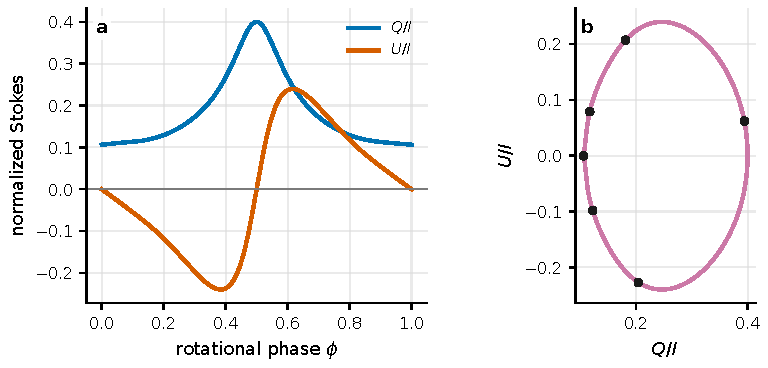
\includegraphics[width=0.92\linewidth]{figures/generated/chapter_11/ch11_stokes_qu_track.pdf}
\caption{旋转磁几何会把偏振角变化投影成 \(Q/I\) 和 \(U/I\) 的相位曲线。左图显示同一相位事件表给出的两个 Stokes 分量，右图显示对应的 Q--U 轨迹；轨迹形状比单独的偏振度更能暴露几何退化和仪器串扰。}
\label{fig:e18-stokes}
\end{figure}

偏振角随相位怎么摆？第一近似用旋转矢量模型（rotating vector model）：

\begin{equation}
  \tan(\psi-\psi_0)=
  \frac{\sin\alpha\,\sin(\phi-\phi_0)}
       {\sin\zeta\cos\alpha-\cos\zeta\sin\alpha\cos(\phi-\phi_0)} .
  \label{eq:e18-rvm}
\end{equation}
\begin{formulaexplain}
\(\psi\)：偏振角；\(\alpha\)：磁轴与自转轴夹角；\(\zeta\)：视线与自转轴夹角；\(\phi\)：自转相位；\(\psi_0,\phi_0\)：零点。它把"偏振角随相位的 S 形摆动"翻译成磁层的几何取向。
\end{formulaexplain}

这个式子最早用于射电脉冲星的偏振几何——它纯粹是把"磁力线投影到天空"的球面三角。但在磁星 X 射线里，它只是一副低维几何骨架，因为表面辐射、共振回旋散射（resonant cyclotron scattering）和真空双折射会一起改写 \(p(E,\phi)\) 和 \(\psi(E,\phi)\)，让实测偏振比纯几何丰富得多 \citep{1969ApL.....3..225R,2018ApJ...854...98W,2011ApJ...730..131F}。

来看一个把这些线索拧在一起的真实例子：磁星 4U 0142+61（图~\ref{fig:e18-biref}）。IXPE 在 \(2\)–\(8\,\mathrm{keV}\) 全带看到线偏振度 \(12\%\pm1\%\)，但分能段看，故事更精彩：低能 \(2\)–\(4\,\mathrm{keV}\) 偏振度 \(14\%\pm1\%\)，高能 \(5.5\)–\(8\,\mathrm{keV}\) 猛升到 \(41\%\pm7\%\)，而中间 \(4\)–\(5\,\mathrm{keV}\) 附近偏振度降到灵敏度下限、偏振角还翻转了约 \(90^\circ\)。这个 \(90^\circ\) 翻转是关键指纹——它意味着两个偏振正常模（O 模、X 模）在这个能量上"接力换班"：低能由一个模主导，高能由另一个模主导，交界处两者相消、方向掉头。源的自转周期 \(P=8.69\,\mathrm{s}\)，磁场 \(B\sim10^{14}\,\mathrm{G}\)，软 X 射线有 \(kT\sim0.5\)–\(1\,\mathrm{keV}\) 的黑体成分，硬尾延伸到几十甚至上百 keV。解释这组数据时，低能 O 模、硬尾 X 模、表面凝聚态或薄大气、共振 Compton 散射都可能参与；\emph{单个}高偏振点还不足以单独判定真空双折射，需要能量、相位、多源一起交叉验证 \citep{2022Sci...378..646T,2023A&A...674L..10C,2023MNRAS.519.3681F}。

\begin{figure}[tbp]
\centering
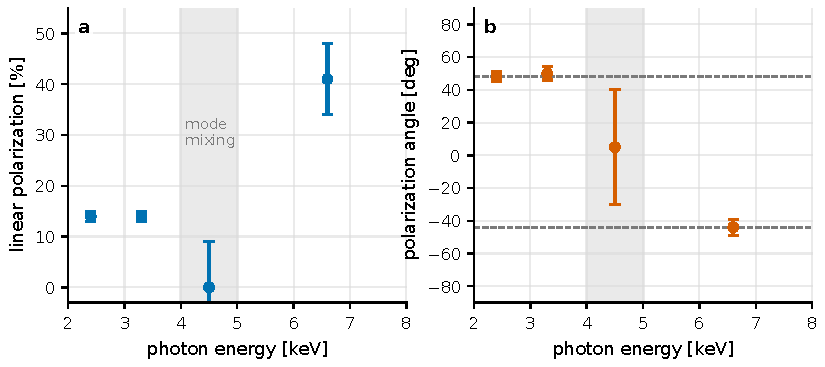
\includegraphics[width=0.92\linewidth]{figures/generated/chapter_11/ch11_birefringence_energy.pdf}
\caption{IXPE 对磁星 4U 0142+61 的结果可以看成两个偏振正常模在能量上的切换。低能 \(2-4\,\mathrm{keV}\) 偏振度约 \(14\%\)，高能 \(5.5-8\,\mathrm{keV}\) 升到约 \(41\%\)，而 \(4-5\,\mathrm{keV}\) 附近偏振度接近最低可探测偏振，偏振角发生约 \(90^\circ\) 翻转。}
\label{fig:e18-biref}
\end{figure}

把这一节收束到本书的大主线上。上面每一步——测 \(\eta_i\)、累加 Stokes、算 \(p\) 与 \(\psi\)、按相位和能量分箱——本质都是在\textbf{偏振通道上做强度/计数统计}。它和第 \ref{chap:e08} 章的 \(g^{(2)}\)、第 \ref{chap:e10} 章的强度干涉是同一族工具：只不过把"两台望远镜"或"两个时刻"换成了"两个偏振基"。第 \ref{chap:e22} 章会把这条"偏振量子通道"正式展开，讨论它在暗物质、轴子等新物理搜寻里的用法；这里的磁星双折射，就是这条通道在强场天体上最干净的一个练兵场。


\section{表面与大气辐射：热斑光变怎样反推中子星半径}
\label{sec:e18-hotspot}

最后回到"分辨不了怎么办"的老问题，但换到中子星上，答案格外漂亮。中子星半径量不到角直径（第 \ref{sec:e18-angsize} 节说过它比白矮星还小），可它偏偏能被测到 \(\sim1\,\mathrm{km}\) 的精度——靠的不是空间分辨，而是\emph{光变形状 + 能谱 + 广义相对论}。核心量是紧致度（compactness）：

\begin{equation}
  u=\frac{2GM}{Rc^2}
  \simeq 0.345
  \left(\frac{M}{1.4\,M_\odot}\right)
  \left(\frac{12\,\mathrm{km}}{R}\right).
  \label{eq:e18-compact}
\end{equation}
\begin{formulaexplain}
\(u\)：紧致度，等于史瓦西半径 \(2GM/c^2\) 与真实半径 \(R\) 之比（无量纲）。\(u\) 越大，引力对光线的弯曲越强，热斑光变的振幅越容易被抹平。
\end{formulaexplain}

物理图像：中子星表面常有一两块比周围热的斑（磁极附近的热斑，hot spot）。星一转，热斑扫过视线，我们看到脉动。可中子星的引力强到能把光线\emph{掰弯}——本来转到背面、该看不见的热斑，发出的光被引力拽回到我们视线里。紧致度越大，掰得越狠，背面的斑也能"漏"过来，于是脉冲的谷底被抬高、振幅被压平。把这个弯曲效应写成一个好用的近似，联系光子离开表面的发射角 \(\alpha\)（这里的 \(\alpha\) 是几何发射角，与前面的精细结构常数 \(\alpha_{\rm fs}\)、旋转矢量模型里的磁轴夹角 \(\alpha\) 同符不同义）和热斑相对视线的中心角 \(\psi\)（这里的 \(\psi\) 是空间角距，不是\eqref{eq:e18-pdop}、\eqref{eq:e18-rvm}里的偏振角 \(\psi\)）：

\begin{equation}
  \cos\alpha\simeq u+(1-u)\cos\psi .
  \label{eq:e18-bending}
\end{equation}
\begin{formulaexplain}
\(\alpha\)：光子离开星面时相对法线的发射角；\(\psi\)：热斑中心相对视线的角距。这个线性近似把"弯曲后一块斑还看不看得见"写成紧致度 \(u\) 的简单函数。
\end{formulaexplain}

它适用于史瓦西外部时空、慢自转到中等自转的标度估算；真正的毫秒脉冲星还要加 Doppler 增亮、光行差、时延、星体扁率和大气束射（beaming）。图~\ref{fig:e18-hotspot} 显示低紧致度时脉冲振幅大、高紧致度时谷底被抬高——半径推断正是利用这种轮廓变化 \citep{2002ApJ...566L..85B,2019AIPC.2127b0008W}。

\begin{figure}[tbp]
\centering
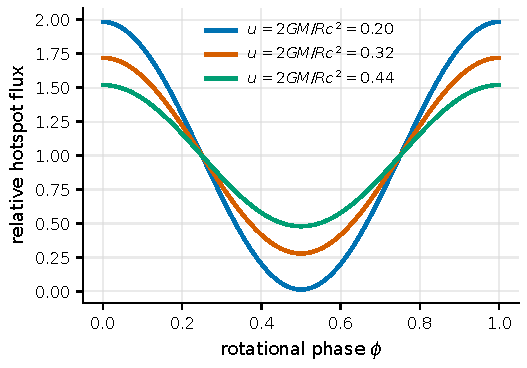
\includegraphics[width=0.78\linewidth]{figures/generated/chapter_11/ch11_hotspot_lightcurve.pdf}
\caption{热斑光变对紧致度很敏感。低紧致度时，斑点转到背面后贡献迅速消失，脉冲振幅大；高紧致度时，引力光弯曲让更大范围的表面可见，光变谷底被抬高。半径推断利用这种轮廓变化，并与质量、倾角、热斑位置和大气束射一起拟合。}
\label{fig:e18-hotspot}
\end{figure}

怎么把这套物理变成对 \(M,R\) 的测量？关键是意识到：我们手里只有一张\emph{事件表}——每个 X 射线光子带一个能量和一个自转相位。把天体模型（热斑几何 + 大气 + 引力弯曲）正向算成"每个能道、每个相位 bin 里该有多少光子"，再和实测比。第 \(j\) 个能道、第 \(k\) 个相位 bin 的期望计数是

\begin{equation}
  \lambda_{jk}(\Theta)=
  T\int dE\,R_j(E)\,
  \left[F_E(\phi_k;\Theta)+B_E\right].
  \label{eq:e18-lambda}
\end{equation}
\begin{formulaexplain}
\(\lambda_{jk}\)：能道 \(j\)、相位 bin \(k\) 的期望计数；\(T\)：曝光时间；\(R_j(E)\)：仪器响应（有效面积 + 能量重分布）；\(F_E\)：热斑模型通量；\(B_E\)：背景。\(\Theta\) 装着 \(M,R\)、距离、倾角、热斑位置等全部参数。它把天体模型翻成探测器里的预期事件数。
\end{formulaexplain}

参数向量 \(\Theta\) 里塞了 \(M,R\)、距离、观测者倾角、热斑经纬度、热斑角半径、温度和大气参数——一整套。实测计数当然不会正好等于 \(\lambda_{jk}\)，它服从泊松统计（第 \ref{chap:e03} 章）：给定期望 \(\lambda\)，观测到 \(N\) 个的概率是 \(e^{-\lambda}\lambda^N/N!\)。把所有能道、相位 bin 的概率乘起来取对数，就是泊松对数似然：

\begin{equation}
  \ln\mathcal{L}(\Theta)=
  \sum_{j,k}\left[
  N_{jk}\ln\lambda_{jk}(\Theta)-\lambda_{jk}(\Theta)-\ln(N_{jk}!)
  \right].
  \label{eq:e18-lnl}
\end{equation}
\begin{formulaexplain}
\(\ln\mathcal{L}\)：泊松对数似然；\(N_{jk}\)：实测计数。把 \(e^{-\lambda}\lambda^N/N!\) 对所有 \((j,k)\) 连乘再取对数就得到它。求半径就是找一组 \(\Theta\)，让所有 \(\lambda_{jk}\) 最贴近事件表。
\end{formulaexplain}

推导只需一步：\(\ln\prod_{jk}\dfrac{e^{-\lambda_{jk}}\lambda_{jk}^{N_{jk}}}{N_{jk}!}=\sum_{jk}\big(-\lambda_{jk}+N_{jk}\ln\lambda_{jk}-\ln N_{jk}!\big)\)。最后一项 \(\ln N_{jk}!\) 不含参数，拟合时是常数、可丢。剩下的就是要\emph{最大化}的目标——这正是第 \ref{chap:e13} 章事件表建模的通用范式，只不过这里的"天体模型"里塞进了引力弯曲和强磁场大气。NICER 对 PSR J0030+0451 和 PSR J0740+6620 的半径测量就是这么做的：J0740 的分析把 NICER 事件表、XMM-Newton 的成像光谱背景、以及射电计时给出的质量和距离先验联合起来，Riley 等得到 \(R=12.39^{+1.30}_{-0.98}\,\mathrm{km}\)、\(M=2.072^{+0.067}_{-0.066}\,M_\odot\)，Miller 等给出方法不同但相容的约束；J0030 的两套独立分析还显示热斑几何可能带复杂的多极磁场结构 \citep{2019ApJ...887L..21R,2019ApJ...887L..24M,2021ApJ...918L..27R,2021ApJ...918L..28M}。请体会这件事的分量：我们没有分辨一个 \(12\,\mathrm{km}\) 的球面（那需要纳角秒级分辨），却把它的半径量到了公里级——纯靠时间、能量和引力光学，把空间信息"折"进了事件表。


\section{本章要点}
\label{sec:e18-summary}

\begin{itemize}
\item \textbf{致密天体靠量子简并撑着，也因此"个头极小"。} 白矮星靠电子简并压（\eqref{eq:e18-pnr}、\eqref{eq:e18-per}）顶住引力，呈"越重越小"的质量–半径关系；但角直径只有微角秒（\eqref{eq:e18-theta}），中子星更小，单口径成像无望——这正把接力棒交给强度干涉（第 \ref{chap:e10} 章）和时间/偏振通道。
\item \textbf{磁场把几何写进相位和偏振。} 磁白矮星的磁层半径与共转半径之比（\eqref{eq:e18-rm}、\eqref{eq:e18-rco}）决定吸积流形态，回旋辐射带来可挑选的偏振信号；中子星的光柱、偶极磁场和自转能损失（\eqref{eq:e18-rlc}–\eqref{eq:e18-edot}）把磁层切成相位坐标，靠相位折叠（\eqref{eq:e18-fold}）读出。
\item \textbf{真空双折射是强场 QED 在偏振上的印记。} 磁星表面 \(B\) 逼近甚至超过临界场 \(B_Q\)（\eqref{eq:e18-bq}），真空变成双折射介质（\eqref{eq:e18-dn}），把星面各处的偏振"梳"齐、抬高净偏振度；4U 0142+61 的能量依赖偏振度和 \(90^\circ\) 偏振角翻转就是这类印记，但需能量、相位、多源交叉验证。
\item \textbf{偏振测量本质是"在偏振基上数光子"。} Stokes 累加（\eqref{eq:e18-stokes}）、偏振度与偏振角（\eqref{eq:e18-pdop}）、旋转矢量模型（\eqref{eq:e18-rvm}）与前面的 \(g^{(2)}\) 同宗同源，是第 \ref{chap:e22} 章"偏振量子通道"的直接前身。
\item \textbf{分辨不了，就把空间信息折进事件表。} 中子星半径靠热斑光变 + 能谱 + 引力弯曲（\eqref{eq:e18-compact}–\eqref{eq:e18-bending}），用泊松似然事件表建模（\eqref{eq:e18-lambda}、\eqref{eq:e18-lnl}）反推，NICER 已把 \(12\,\mathrm{km}\) 的中子星量到公里级。
\end{itemize}

\noindent\textbf{想一想。}
（1）为什么白矮星"越重越小"，而普通主序星"越重越大"？从简并压指数 \(5/3\to4/3\) 的软化去想。
（2）如果真空双折射\emph{不存在}，磁星的净偏振度会偏高还是偏低？为什么"一个高偏振度"能当作双折射的间接证据？
（3）中子星半径只有 \(12\,\mathrm{km}\)、角直径远小于任何望远镜的分辨极限，我们却测得出它的半径——被测量的"信息"到底藏在观测数据的哪个维度里？
